\documentclass{article}
%DIF LATEXDIFF DIFFERENCE FILE



\usepackage[left=3cm, right=3cm, top=3cm, bottom=3cm]{geometry}
\usepackage{pdfpages}
\usepackage{cite}
\usepackage{eurosym}
\usepackage[utf8]{inputenc}
\usepackage{graphicx}
\usepackage{amssymb}
\usepackage{amsmath}
\usepackage{array}
\usepackage{graphicx}
%DIF 13a13-16
 %DIF > 
\usepackage{breakurl} %DIF > 
\usepackage[breaklinks]{hyperref} %DIF > 
 %DIF > 
%DIF -------
\usepackage{apacite}
\usepackage{gensymb}

%DIF 16a20-27
\usepackage{titlesec} %DIF > 
 %DIF > 
\setcounter{secnumdepth}{4} %DIF > 
 %DIF > 
\titleformat{\paragraph} %DIF > 
{\normalfont\normalsize\bfseries}{\theparagraph}{1em}{} %DIF > 
\titlespacing*{\paragraph} %DIF > 
{0pt}{3.25ex plus 1ex minus .2ex}{1.5ex plus .2ex} %DIF > 
%DIF -------
\graphicspath{ {./verslag_figuren/} }

\usepackage[numbib]{tocbibind}

%%%%% voor implementeren matlabcode in latex %%%%%

\usepackage{listings}
\usepackage{color} %red, green, blue, yellow, cyan, magenta, black, white
\definecolor{mygreen}{RGB}{28,172,0} % color values Red, Green, Blue
\definecolor{mylilas}{RGB}{170,55,241} 

%%%%%%%%%%%%%%%%%%%%%%%%%%%%%%%%%%%%%%%%%%%%%%%%%%
%DIF PREAMBLE EXTENSION ADDED BY LATEXDIFF
%DIF UNDERLINE PREAMBLE %DIF PREAMBLE
\RequirePackage[normalem]{ulem} %DIF PREAMBLE
\RequirePackage{color}\definecolor{RED}{rgb}{1,0,0}\definecolor{BLUE}{rgb}{0,0,1} %DIF PREAMBLE
\providecommand{\DIFaddtex}[1]{{\protect\color{blue}\uwave{#1}}} %DIF PREAMBLE
\providecommand{\DIFdeltex}[1]{{\protect\color{red}\sout{#1}}}                      %DIF PREAMBLE
%DIF SAFE PREAMBLE %DIF PREAMBLE
\providecommand{\DIFaddbegin}{} %DIF PREAMBLE
\providecommand{\DIFaddend}{} %DIF PREAMBLE
\providecommand{\DIFdelbegin}{} %DIF PREAMBLE
\providecommand{\DIFdelend}{} %DIF PREAMBLE
%DIF FLOATSAFE PREAMBLE %DIF PREAMBLE
\providecommand{\DIFaddFL}[1]{\DIFadd{#1}} %DIF PREAMBLE
\providecommand{\DIFdelFL}[1]{\DIFdel{#1}} %DIF PREAMBLE
\providecommand{\DIFaddbeginFL}{} %DIF PREAMBLE
\providecommand{\DIFaddendFL}{} %DIF PREAMBLE
\providecommand{\DIFdelbeginFL}{} %DIF PREAMBLE
\providecommand{\DIFdelendFL}{} %DIF PREAMBLE
%DIF HYPERREF PREAMBLE %DIF PREAMBLE
\providecommand{\DIFadd}[1]{\texorpdfstring{\DIFaddtex{#1}}{#1}} %DIF PREAMBLE
\providecommand{\DIFdel}[1]{\texorpdfstring{\DIFdeltex{#1}}{}} %DIF PREAMBLE
\newcommand{\DIFscaledelfig}{0.5}
%DIF HIGHLIGHTGRAPHICS PREAMBLE %DIF PREAMBLE
\RequirePackage{settobox} %DIF PREAMBLE
\RequirePackage{letltxmacro} %DIF PREAMBLE
\newsavebox{\DIFdelgraphicsbox} %DIF PREAMBLE
\newlength{\DIFdelgraphicswidth} %DIF PREAMBLE
\newlength{\DIFdelgraphicsheight} %DIF PREAMBLE
% store original definition of \includegraphics %DIF PREAMBLE
\LetLtxMacro{\DIFOincludegraphics}{\includegraphics} %DIF PREAMBLE
\newcommand{\DIFaddincludegraphics}[2][]{{\color{blue}\fbox{\DIFOincludegraphics[#1]{#2}}}} %DIF PREAMBLE
\newcommand{\DIFdelincludegraphics}[2][]{% %DIF PREAMBLE
\sbox{\DIFdelgraphicsbox}{\DIFOincludegraphics[#1]{#2}}% %DIF PREAMBLE
\settoboxwidth{\DIFdelgraphicswidth}{\DIFdelgraphicsbox} %DIF PREAMBLE
\settoboxtotalheight{\DIFdelgraphicsheight}{\DIFdelgraphicsbox} %DIF PREAMBLE
\scalebox{\DIFscaledelfig}{% %DIF PREAMBLE
\parbox[b]{\DIFdelgraphicswidth}{\usebox{\DIFdelgraphicsbox}\\[-\baselineskip] \rule{\DIFdelgraphicswidth}{0em}}\llap{\resizebox{\DIFdelgraphicswidth}{\DIFdelgraphicsheight}{% %DIF PREAMBLE
\setlength{\unitlength}{\DIFdelgraphicswidth}% %DIF PREAMBLE
\begin{picture}(1,1)% %DIF PREAMBLE
\thicklines\linethickness{2pt} %DIF PREAMBLE
{\color[rgb]{1,0,0}\put(0,0){\framebox(1,1){}}}% %DIF PREAMBLE
{\color[rgb]{1,0,0}\put(0,0){\line( 1,1){1}}}% %DIF PREAMBLE
{\color[rgb]{1,0,0}\put(0,1){\line(1,-1){1}}}% %DIF PREAMBLE
\end{picture}% %DIF PREAMBLE
}\hspace*{3pt}}} %DIF PREAMBLE
} %DIF PREAMBLE
\LetLtxMacro{\DIFOaddbegin}{\DIFaddbegin} %DIF PREAMBLE
\LetLtxMacro{\DIFOaddend}{\DIFaddend} %DIF PREAMBLE
\LetLtxMacro{\DIFOdelbegin}{\DIFdelbegin} %DIF PREAMBLE
\LetLtxMacro{\DIFOdelend}{\DIFdelend} %DIF PREAMBLE
\DeclareRobustCommand{\DIFaddbegin}{\DIFOaddbegin \let\includegraphics\DIFaddincludegraphics} %DIF PREAMBLE
\DeclareRobustCommand{\DIFaddend}{\DIFOaddend \let\includegraphics\DIFOincludegraphics} %DIF PREAMBLE
\DeclareRobustCommand{\DIFdelbegin}{\DIFOdelbegin \let\includegraphics\DIFdelincludegraphics} %DIF PREAMBLE
\DeclareRobustCommand{\DIFdelend}{\DIFOaddend \let\includegraphics\DIFOincludegraphics} %DIF PREAMBLE
\LetLtxMacro{\DIFOaddbeginFL}{\DIFaddbeginFL} %DIF PREAMBLE
\LetLtxMacro{\DIFOaddendFL}{\DIFaddendFL} %DIF PREAMBLE
\LetLtxMacro{\DIFOdelbeginFL}{\DIFdelbeginFL} %DIF PREAMBLE
\LetLtxMacro{\DIFOdelendFL}{\DIFdelendFL} %DIF PREAMBLE
\DeclareRobustCommand{\DIFaddbeginFL}{\DIFOaddbeginFL \let\includegraphics\DIFaddincludegraphics} %DIF PREAMBLE
\DeclareRobustCommand{\DIFaddendFL}{\DIFOaddendFL \let\includegraphics\DIFOincludegraphics} %DIF PREAMBLE
\DeclareRobustCommand{\DIFdelbeginFL}{\DIFOdelbeginFL \let\includegraphics\DIFdelincludegraphics} %DIF PREAMBLE
\DeclareRobustCommand{\DIFdelendFL}{\DIFOaddendFL \let\includegraphics\DIFOincludegraphics} %DIF PREAMBLE
%DIF LISTINGS PREAMBLE %DIF PREAMBLE
\RequirePackage{listings} %DIF PREAMBLE
\RequirePackage{color} %DIF PREAMBLE
\lstdefinelanguage{DIFcode}{ %DIF PREAMBLE
%DIF DIFCODE_UNDERLINE %DIF PREAMBLE
  moredelim=[il][\color{red}\sout]{\%DIF\ <\ }, %DIF PREAMBLE
  moredelim=[il][\color{blue}\uwave]{\%DIF\ >\ } %DIF PREAMBLE
} %DIF PREAMBLE
\lstdefinestyle{DIFverbatimstyle}{ %DIF PREAMBLE
	language=DIFcode, %DIF PREAMBLE
	basicstyle=\ttfamily, %DIF PREAMBLE
	columns=fullflexible, %DIF PREAMBLE
	keepspaces=true %DIF PREAMBLE
} %DIF PREAMBLE
\lstnewenvironment{DIFverbatim}{\lstset{style=DIFverbatimstyle}}{} %DIF PREAMBLE
\lstnewenvironment{DIFverbatim*}{\lstset{style=DIFverbatimstyle,showspaces=true}}{} %DIF PREAMBLE
%DIF END PREAMBLE EXTENSION ADDED BY LATEXDIFF

\begin{document}

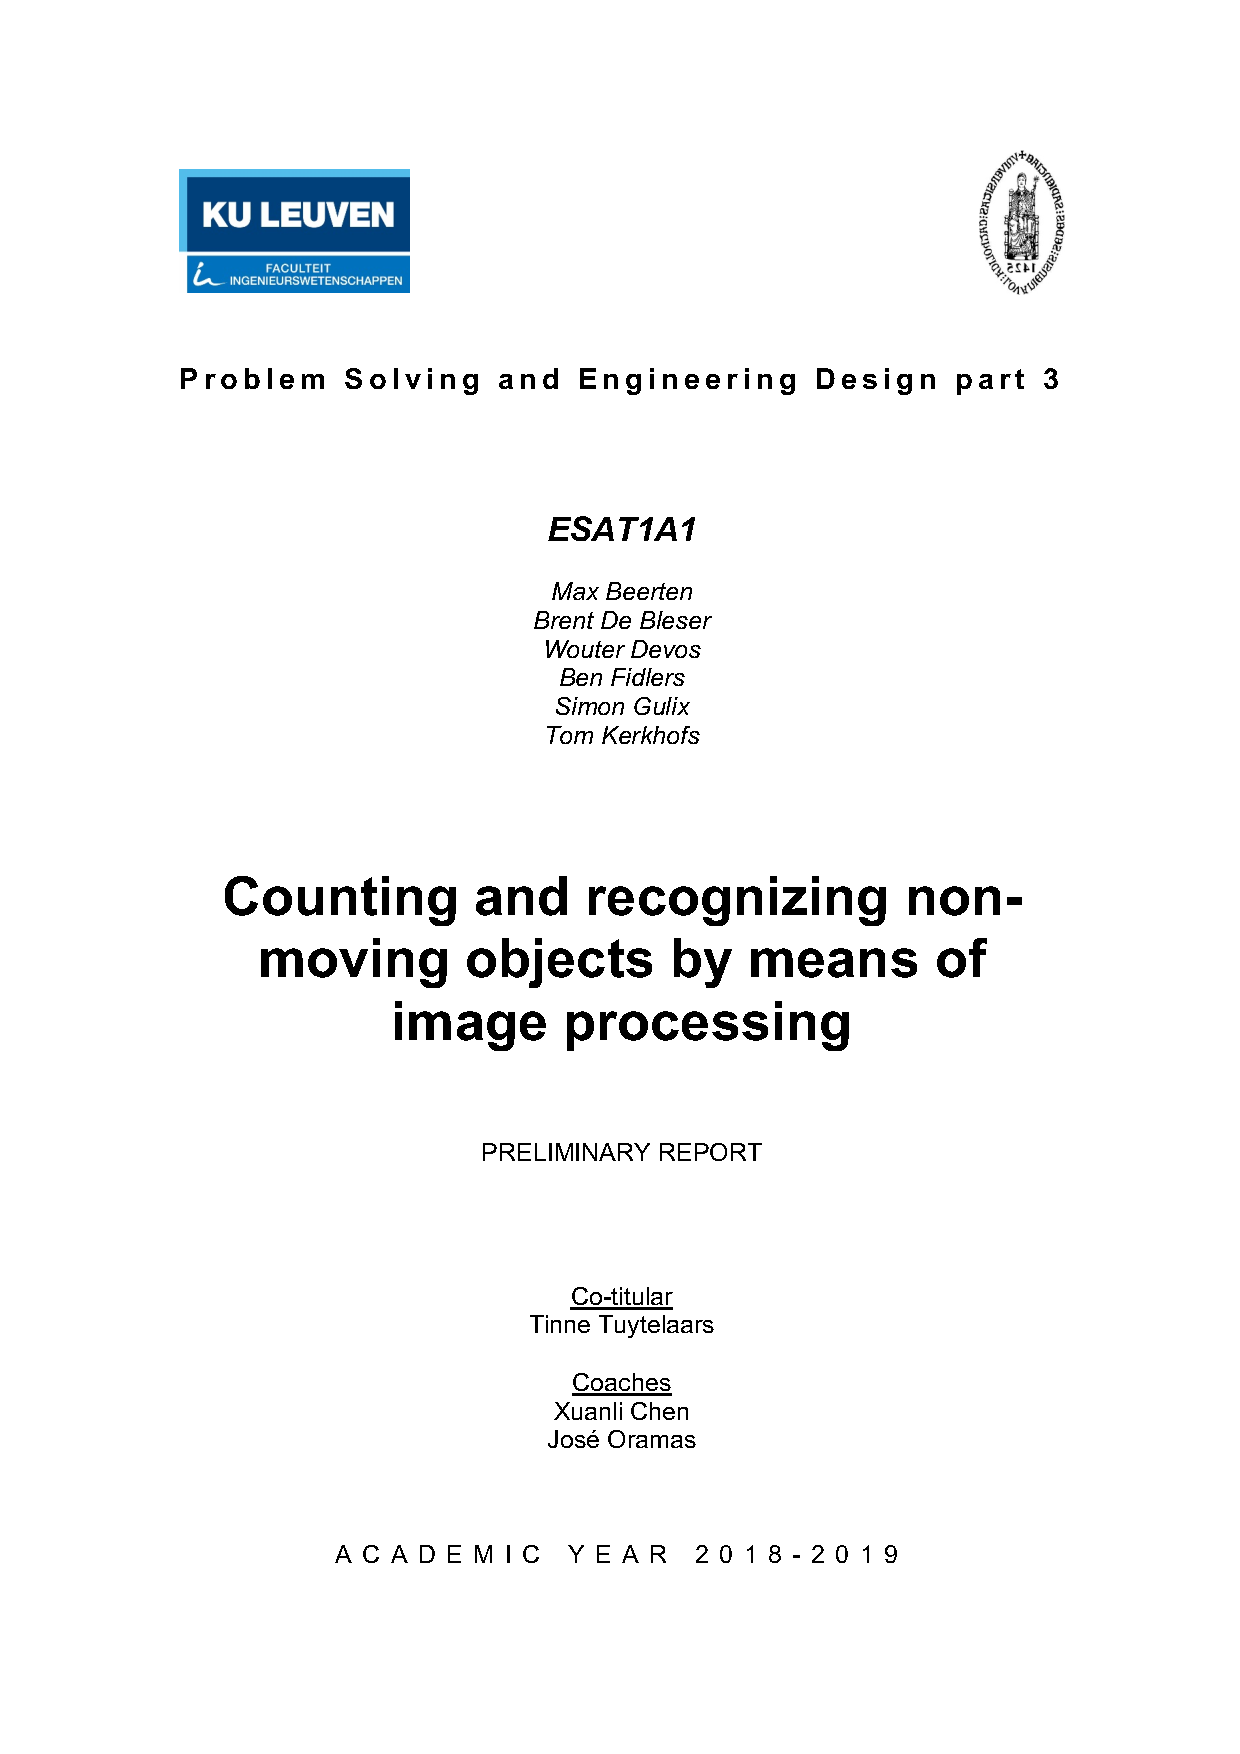
\includepdf[pages=-]{frontpage.pdf}

\newpage
\tableofcontents
\DIFdelbegin %DIFDELCMD < \thispagestyle{empty}
%DIFDELCMD < %%%
\DIFdelend \DIFaddbegin \pagenumbering{roman}
\DIFaddend 

%\newpage
%\listoftables
%\thispagestyle{empty}

\newpage
\listoffigures
\DIFdelbegin %DIFDELCMD < \thispagestyle{empty}
%DIFDELCMD < %%%
\DIFdelend 

\newpage
\section{Introduction}
\pagenumbering{arabic}
Digital image processing has been a crucial part of the current digitalisation movement. From industrial machinery to customer amusement, the vision of computer-aided systems has become a given for most users. While image alteration and manipulation remain a core part of this field of study, nowadays other image related problems are being solved by artificial intelligence. Most were considered to be an important part of digital image processing. Among these, the problem of this paper can be found: feature extraction. The ability to count objects in an image, to be more exact. So why use 'traditional' methods to solve this problem? While being a great way for unravelling many problems, artificial intelligence mostly provides general solutions. However, certain cases are solved more efficiently by specific schemes. Such is the case with object counting: while deep learning algorithms need a big data set as training material, standard image processing only requires the image itself.\\
Regardless which way a method processes images, it needs a visual source. In this paper the focus is on live object counting, which is only possible with a camera. Evidently, the choice of hardware greatly impacts the methods that can be used. This choice will be covered in section 3.1: Hardware.\\
By far the most important part of this task is the algorithm by which the items in the picture will be numbered. Classically, object counting algorithms have a standard group of steps: filtering, converting to an intensity matrix, edge detection, converting to a binary matrix, boundary boxing and the counting itself. These segments don't have a fixed order and can occur multiple times in the final method. Most of these steps can also be approached in different ways. A wide range of possible filters, kernels, edge detection methods, etc. exist, which all have their benefits and drawbacks\DIFdelbegin \DIFdel{\mbox{%DIFAUXCMD
\cite{dirac}}\hspace{0pt}%DIFAUXCMD
}\DIFdelend . These choices will be discussed in section 3.2: Software.\\
These methods, while being the core of the solution, are fairly simple to implement with the use of libraries or built-in functions. In this paper is opted to give a full implementation of these functions, limiting the usage of libraries to the minimum. If the functions are deemed to be basic, only a simple explanation will be given.

\section{Problem Description}
The object counting system described in this report is capable of counting non-moving objects in a basket. These objects can vary in shape, size and colour. Thus, the colour of both the basket and its contents are free from restrictions.\\
In the primary stage of this paper, not all these variables are taken into account\DIFdelbegin \DIFdel{, with the }\DIFdelend \DIFaddbegin \DIFadd{. The }\DIFaddend simplest objects, which the system is required to count, being rectangles, cylinders and circles, all with a uniform colour. If possible, the circumference of these objects can be outlined and measured as shown in Fig.~\ref{fig:example}.\\ All of this is done in real-time and with a budget of \euro 250.
\begin{figure}[h]
\centering
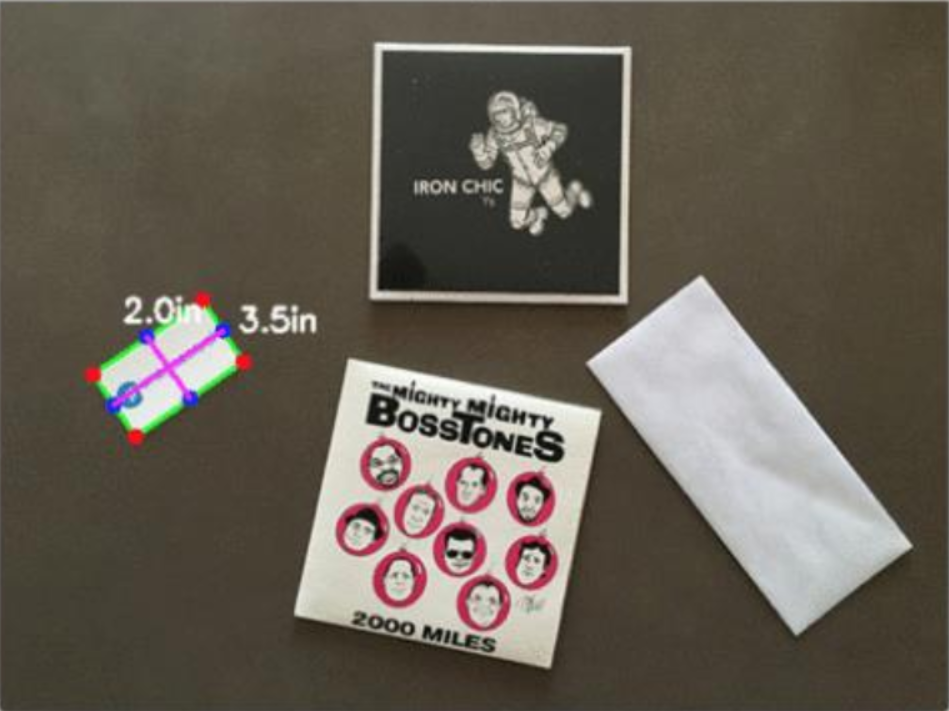
\includegraphics[width=0.7\linewidth]{opdracht.png}
\caption{Example of a possible result.}
\label{fig:example}
\end{figure}

\section{Design}
\subsection{Hardware}
The hardware to create a system as described above, is not complicated. In essence, it consists of a computer, a camera and a cable to transfer the data between the \DIFdelbegin \DIFdel{latter two}\DIFdelend \DIFaddbegin \DIFadd{prior named necessities}\DIFaddend . Each of these hardware components is discussed in the following section.\\
Choosing the camera is a vital element in this project. If chosen poorly, it can fiercely limit the outcome of the final algorithm. There are three main options for visual input: an ordinary webcam, an industrial camera or a camera with built-in depth sensors. Each with its pros and cons. A webcam is cheap and readily available but does not assure good image quality and easy access to its data. A camera for industrial usage is rather expensive, especially \DIFdelbegin \DIFdel{with a }\DIFdelend \DIFaddbegin \DIFadd{considering the }\DIFaddend budget of \euro 250. Industrial grade options which are cheap enough \DIFdelbegin \DIFdel{do }\DIFdelend exist, but these models deliver their images in greyscale. This greatly limits the possible methods which can be used. Thirdly, the depth sensing cameras are available in a reasonable price range and deliver, overall, good quality data. Moreover these models have the added benefit of \DIFaddbegin \DIFadd{a }\DIFaddend depth sensor which, in contrast to the previous \DIFdelbegin \DIFdel{option}\DIFdelend \DIFaddbegin \DIFadd{options}\DIFaddend , adds more possible ways to solve the problem.\\
Having considered all of the above, the best option is the latter one. More specifically, the system described in this report is based on a Kinect V2 from Microsoft. This camera has a \DIFdelbegin \DIFdel{color }\DIFdelend \DIFaddbegin \DIFadd{colour }\DIFaddend lens with a resolution of $1920$ by $1080$ pixels and a corresponding field of view of $84.1\degree$ by $53.8\degree$\cite{kinect_specifications}. The high resolution ensures an accurate matrix representation of the real image. Each \DIFdelbegin \DIFdel{color }\DIFdelend \DIFaddbegin \DIFadd{colour }\DIFaddend frame pulled from the Kinect V2 is represented by an array structure of $1080$x$1920$x$3$. Every element corresponds with a pixel of the image and varies between $0$ and $255$. Obviously it can be separated into three different matrices each belonging to $\mathbb{R}^{2}$ and based on a different colour: red, green or blue.\\ Next to the colour camera, the Kinect also possesses a depth sensor. An infrared projector and camera make this possible\cite{kinect_v2}. It provides a $424$x$512$ array making the depth image one of roughly $200 000$ pixels. The field of view of this function is $70.6\degree$ by $60\degree$. Note that the depth camera provides data about parts of the environment that the \DIFdelbegin \DIFdel{color }\DIFdelend \DIFaddbegin \DIFadd{colour }\DIFaddend camera does not see, and vice versa. When the computer reads the depth data, every number in the matrix represents a distance in millimetres. Obviously there are some restrictions. This technology only provides correct information if the object is at a distance located in between 0.5m to 4m. This has to be taken into account for further implementation of this paper.\\
As second element of hardware the computer has a less important role. Preferably, OSX isn't used as operating system for this application, because the Kinect drivers do not exist for Macintosh computers. If the reader has a Mac, problems can be avoided by running either Windows or Ubuntu on a virtual machine. The algorithm should run in an acceptable time frame on every machine.\\
To conclude this section a brief word on the necessary transfer cable. Since a depth sensing camera is used, two types of data (depth and \DIFdelbegin \DIFdel{color}\DIFdelend \DIFaddbegin \DIFadd{colour}\DIFaddend ) need to be transferred. The Microsoft OEM Kinect Adapter makes this possible. \DIFdelbegin \DIFdel{The }\DIFdelend \DIFaddbegin \DIFadd{This }\DIFaddend special adapter is the only available option and consists of two general parts. One part for delivering current to the camera and the other to transfer both types of data to the connected computer.

\subsection{Software}
There are a lot of options when it comes to software and a wide range of different algorithms for image processing exist. The diagram in \DIFdelbegin \DIFdel{appendix C }\DIFdelend \DIFaddbegin \DIFadd{Appendix A }\DIFaddend shows a couple of different methods. But keep in mind \DIFaddbegin \DIFadd{that }\DIFaddend there is no \DIFdelbegin \DIFdel{'right }\DIFdelend \DIFaddbegin \DIFadd{‘right }\DIFaddend way’ to count \DIFaddbegin \DIFadd{the number of }\DIFaddend objects in an image
\DIFdelbegin \DIFdel{.
}\DIFdelend 

\subsubsection{\DIFdelbegin \DIFdel{Analysis RGB image}\DIFdelend \DIFaddbegin \DIFadd{Analysing different methods}\DIFaddend }
Analysing RGB images is a creative process. Different approaches have their own advantages and disadvantages. The only general ideas that are common throughout most algorithms are:
\begin{itemize}
\item Converting the RGB image to greyscale
\item Run filters over the image to remove noise
\item Transforming the image to a binary image
\end{itemize}
In the next scope, three general methods are featured and briefly discussed. Each was investigated in prospect of this paper.
\paragraph{Method 1}
\DIFdelbegin \DIFdel{\mbox{}}\DIFdelend \DIFaddbegin 

\textit{\DIFadd{The image first passes through an threshold algorithm. After that there is an algorithm to find the edges of an object.}}\DIFaddend \\ 
This method is the most simple and straightforward to implement. \DIFdelbegin \DIFdel{There are two ways to approach this. The }\DIFdelend \DIFaddbegin \DIFadd{the first step. Either the }\DIFaddend image can be converted to a greyscale one which is analysed or the image can be analysed in its three different spectra (red, green and blue) which are combined afterwards. In the next step \DIFdelbegin \DIFdel{it }\DIFdelend \DIFaddbegin \DIFadd{the array }\DIFaddend is passed trough a thresholding algorithm with a pre-defined threshold value. The output is a binary matrix. Thus, this array only has 0's and 1's as elements, representing the colours black and white, respectively. When in possession of a truly black and white image, a simple edge detection program is run which makes the edges visible.\\
The key to solving the problem in this specific scheme is writing code that finds the threshold value based on environmental parameters. An example of such an algorithm is the imbinarize function from the \DIFdelbegin \DIFdel{Processing Toolbox }\DIFdelend \DIFaddbegin \DIFadd{processing toolbox }\DIFaddend \cite{Mathworks}. This function is based on the Otsu's method. An example of a program that uses this function can be found in Appendix \DIFdelbegin \DIFdel{A}\DIFdelend \DIFaddbegin \DIFadd{B \mbox{%DIFAUXCMD
\cite{threshold}}\hspace{0pt}%DIFAUXCMD
}\DIFaddend .
\\Advantages: It’s an easy and fast algorithm.
\\Disadvantages: With a pre-defined threshold value it just classifies pixels based on colour. A dynamic value is required.
\paragraph{Method 2}
\DIFdelbegin \DIFdel{\mbox{}}\DIFdelend \DIFaddbegin \textit{\DIFadd{This method is the opposite of method 1. It starts with finding edges and than a threshold algorithm at last}}\DIFaddend \\
The second method tackles the colour analysis in the opposite order than the first method, as it commences with an edge detection algorithm. Since the input image is still very complex, it is first converted to a filtered greyscale image. Still, this edge detection is more comprehensive than \DIFdelbegin \DIFdel{that one }\DIFdelend \DIFaddbegin \DIFadd{the corresponding code }\DIFaddend from method one. The output is still a greyscale image, contrary to the binary array the reader might expect. This is followed by some thresholding code with a pre-defined threshold value. The current image is now represented by a matrix where the edges are outlined using binary elements.
\\Advantages: It detects all kinds of objects, not based on colour or shape.
\\Disadvantages: The boundary between different objects needs to be clear for this to work.
\paragraph{Method 3}
\DIFdelbegin \DIFdel{\mbox{}}\DIFdelend \DIFaddbegin \textit{\DIFadd{This method compares the image to an image of the background and uses that to threshold the image and finding the outline of objects.}}\DIFaddend \\
The third way takes a different approach to solving the analysis of the colour image. Instead of looking at the objects\DIFaddbegin \DIFadd{, }\DIFaddend the algorithm looks for the background. This is possible in two different ways and both \DIFdelbegin \DIFdel{ways }\DIFdelend make a compromise in functionality. The first way needs a picture of the empty background without any objects. The second way looks for \DIFdelbegin \DIFdel{the most common pixels }\DIFdelend \DIFaddbegin \DIFadd{a pre-defined range which contains more pixels than other ranges}\DIFaddend . The compromise \DIFdelbegin \DIFdel{here }\DIFdelend \DIFaddbegin \DIFadd{of the second named perspective }\DIFaddend is the fact that there can't be too much objects in the image. After applying filters the program loops through the image pixel by pixel. This necessary but time consuming loop checks if the pixel on the image is more or less the same as the corresponding pixel of the background image. If located within a pre-determined range\DIFdelbegin \DIFdel{, }\DIFdelend \DIFaddbegin \DIFadd{: }\DIFaddend that element of the array gets classified as background. The consequence is that the output is a binary image with clear-cut objects. An example of this implementation can be found in Appendix \DIFdelbegin \DIFdel{B}\DIFdelend \DIFaddbegin \DIFadd{C}\DIFaddend . 
\\Advantages: It is very good in detecting objects, not being based on colour or shape.
\\Disadvantages: There needs to be an image of the empty background or the image need to be a big part of your image and has to be consistent. On top of that the lighting conditions and shadow play a big part. 
\DIFdelbegin \paragraph{\DIFdel{Choice of method}}%DIFAUXCMD
\addtocounter{paragraph}{-1}%DIFAUXCMD
\DIFdelend \DIFaddbegin \subsubsection{\DIFadd{Choice of method}}\DIFaddend \mbox{}\\
After comparing these different schemes, the second method comes out as the better of the three. See Fig. \ref{fig:comparison_methods} for the comparison.\\ The \DIFaddbegin \DIFadd{actual code of this function can be found in Appendix D. 
}\paragraph{\DIFadd{Step 1: converting to greyscale}}
\DIFadd{The }\DIFaddend first step, as discussed above, is to convert the image to greyscale \cite{greyscale}. This is easily done by calculating a weighted average of the values of all three red, green and blue matrices as shown in the following equation.
\begin{figure}[h]
\center
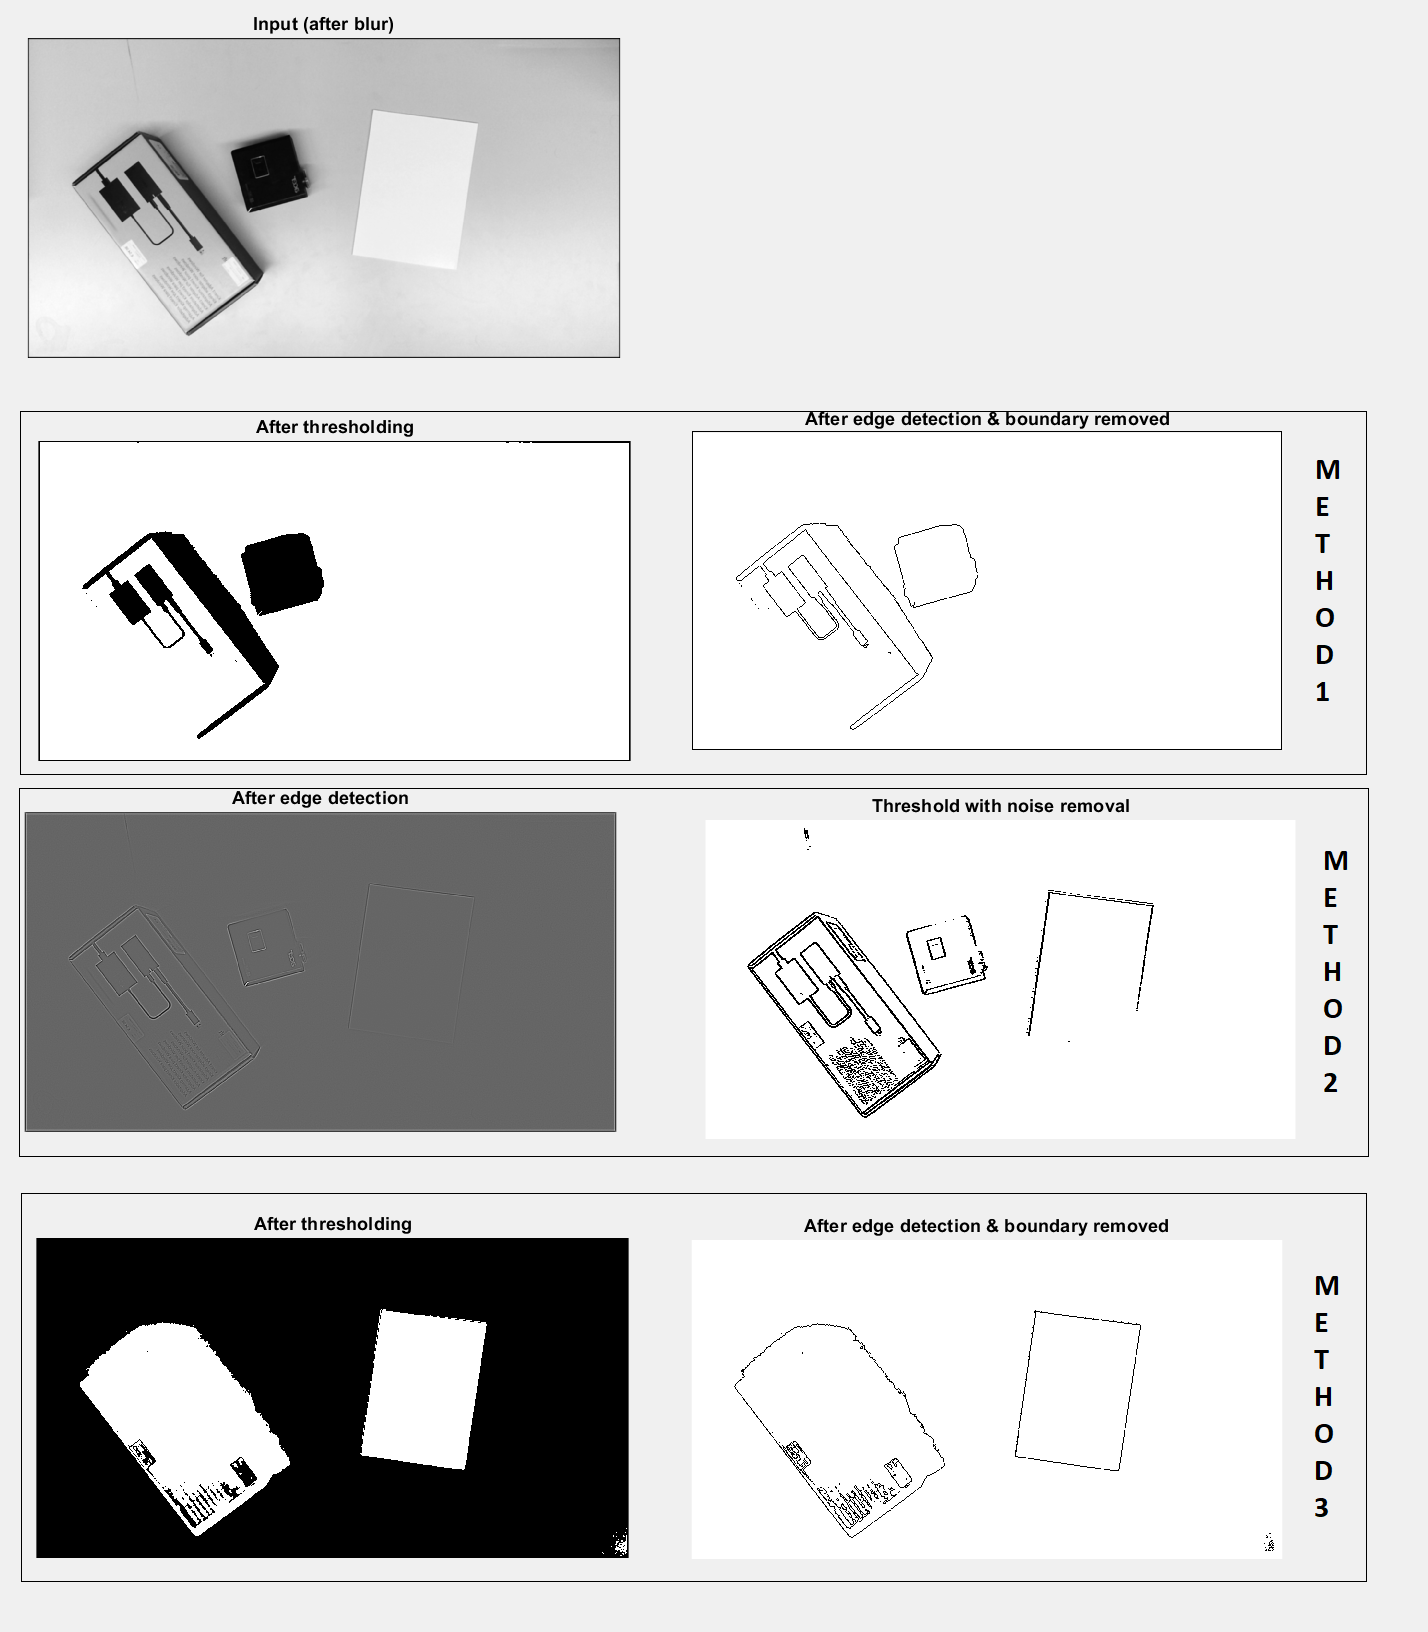
\includegraphics[width=0.7\linewidth]{comparison_methods.png}
\caption{A comparison between the 3 different methods.}
\label{fig:comparison_methods}
\end{figure}
\begin{equation}
greyscale\_image(row, col) = 0.2989 * RED + 0.5870 * GREEN + 0.1140 * BLUE
\end{equation}
The used coefficients add up to $1$. This has to be the case, if else some values could exceed the $0$ to $255$ range. All these values $greyscale\_image(row, col)$ form the new image.
\DIFdelbegin %DIFDELCMD < \noindent %%%
\DIFdelend \DIFaddbegin \paragraph{\DIFadd{Step 2: filtering the image}}
\DIFaddend Before running the image through an edge detection algorithm, two filters are applied. Both blur the image to an extent such that noise after edge detection is considerably reduced. This effect is visualised in Fig. \ref{fig:filter_comparison}\DIFaddbegin \DIFadd{.
}\DIFaddend Firstly a Gaussian blur\cite{gaussian} is applied. Most filters are a convolution of a kernel with the image. For a Gaussian blur the kernel G, found below, is used. This is just a weighted average. This has as consequence that the elements centred around the main pixel have bigger weights than those at the edges.
\begin{figure}[h]
\center
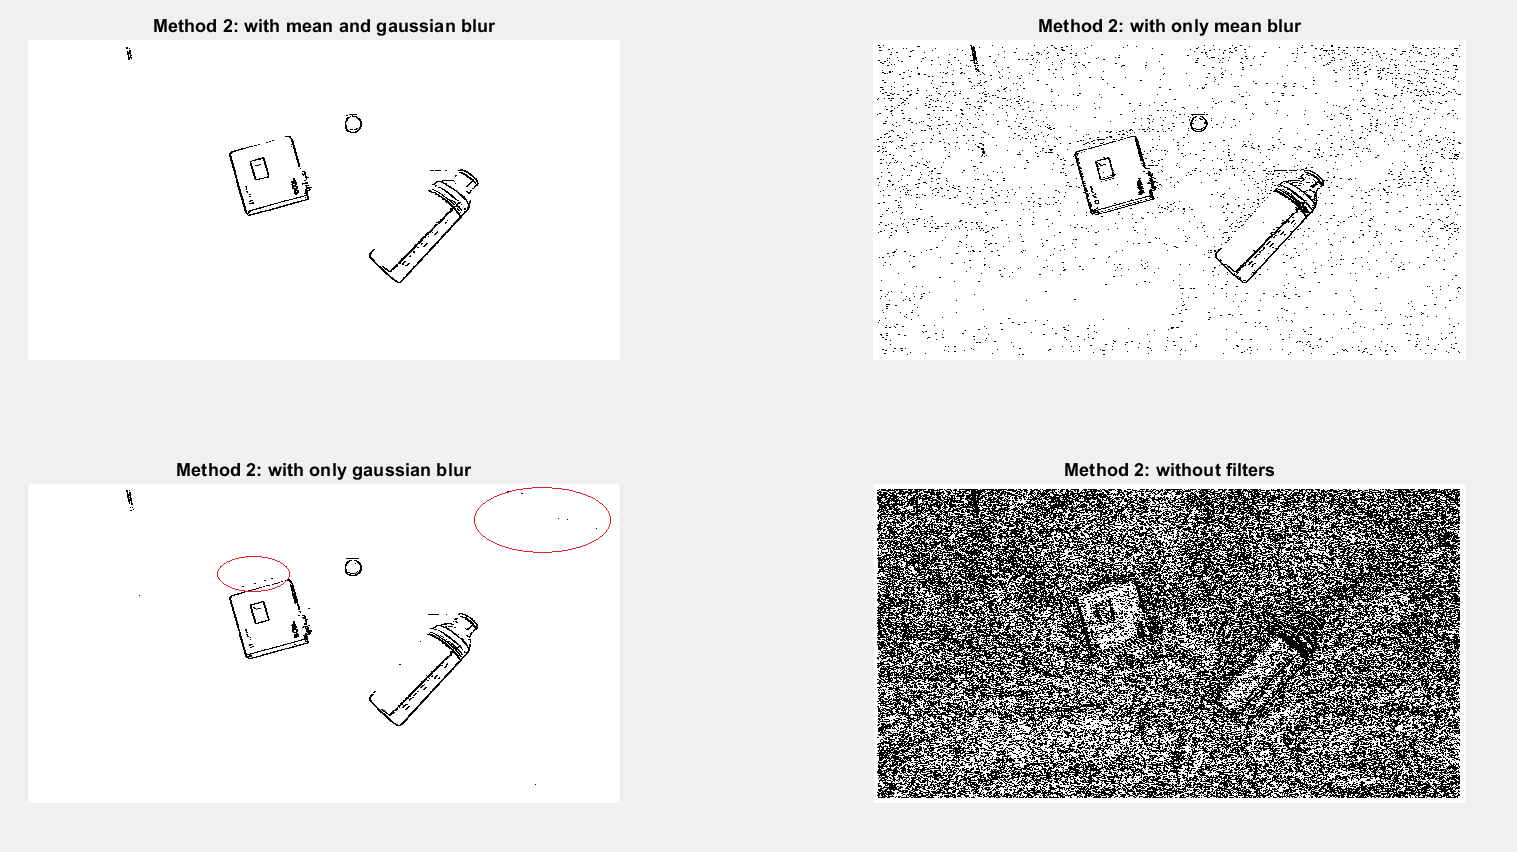
\includegraphics[width=0.7\linewidth]{filter_comparison.png}
\caption{A comparison with the use of filters.}
\label{fig:filter_comparison}
\end{figure}
\begin{equation}
G = (1/159) * 
\begin{bmatrix}
2 & 4 & 5 & 4 & 2\\
4 & 9 & 12 & 9 & 4\\
5 & 12 & 15 & 12 & 5\\
4 & 9 & 12 & 9& 4\\
2 & 4 & 5 & 4 & 2
\end{bmatrix}
\end{equation}
The second blur is a mean blur \cite{mean}. This is almost the same, the actions are just done with a different kernel\DIFdelbegin \DIFdel{kernel}\DIFdelend . This kernel calculates the average of the values around the pixel.
\begin{equation}
M = (1/9) * 
\begin{bmatrix}
1&1&1\\
1&1&1\\
1&1&1
\end{bmatrix}
\end{equation}
Note that both G and M have a norm of 1. If this wasn't the case, pixel values of the filtered image could exceed the boundary values of 0 to 255 for uint8 numbers. 
\DIFdelbegin %DIFDELCMD < \\
%DIFDELCMD < %%%
\DIFdelend \DIFaddbegin \paragraph{\DIFadd{Step 3: edge detection}}
\DIFaddend After both filters are applied, the image is ready to be run through an edge detection algorithm\cite{edge_detection}. This algorithm is on itself also a filter with kernel given by the matrix L shown below.
It calculates the \textit{spatial derivative} or in simpler words, it highlights regions of rapid intensity change.
\begin{equation}
L =\begin{bmatrix}
0&-1&0\\
-1&4&-1\\
0&-1&0
\end{bmatrix}
\end{equation}
\noindent Note now how the kernel uses the pixels next to the evaluated pixel to see how much intensity changes. If the image wouldn't have been filtered before convolution with L, more 'edges' would have been drawn because more irregular areas exist.\\
Note also how this convolution returns a new image which can have negative values for its pixels. The more negative the value, the darker the image. To make this possible\DIFaddbegin \DIFadd{, }\DIFaddend a different number type is used.
\DIFdelbegin %DIFDELCMD < \\
%DIFDELCMD < %%%
\DIFdelend \DIFaddbegin \paragraph{\DIFadd{Step 4: threshold}}
\DIFaddend The threshold algorithm, used in the following step, is based on this feature. This algorithm runs through \DIFdelbegin \DIFdel{to }\DIFdelend \DIFaddbegin \DIFadd{the }\DIFaddend whole matrix and assigns each value \DIFdelbegin \DIFdel{with }\DIFdelend \DIFaddbegin \DIFadd{to }\DIFaddend either a 0 or a 1. It decides this by assessing if the current value is either smaller than or bigger than a threshold value, respectively. After conducting multiple experiments and testing, a threshold value of 2 seems to do the trick. A more dynamic way of determining this value may be developed in the next weeks. After applying this edge detection, the matrix becomes a binary image with only the edges in white. Based on these edges\DIFaddbegin \DIFadd{, }\DIFaddend it is possible to outline the objects and count them. More on these functionalities can be found  in section 4: Research. 

\subsubsection{Analysis Depth Sensor}
Using only the RGB image does have some shortcomings\DIFdelbegin \DIFdel{. It }\DIFdelend \DIFaddbegin \DIFadd{, for example, it }\DIFaddend is rather difficult to distinguish an object from its shadow, a multicoloured object could be seen as multiple different objects and a lot of reflection could make an object undetectable. These are some of the reasons why enrichening the object counting algorithm with the usage of a depth sensor is advised. Like featured in the section about the hardware, each element of the input data represents a distance in millimeters.\\
Firstly the code should be able to provide a clear difference in height between the objects and the background using the depth data. This is followed \DIFdelbegin \DIFdel{with }\DIFdelend \DIFaddbegin \DIFadd{by }\DIFaddend a filter to get rid of the existing noise\DIFdelbegin \DIFdel{reduction}\DIFdelend . At last, the filtered matrix will be used to detect the edges of the objects and thus detect the items themselves. The code that accompanies this description, can be found in appendix \DIFdelbegin \DIFdel{B}\DIFdelend \DIFaddbegin \DIFadd{E}\DIFaddend .

\paragraph{Detection of the difference in height}\mbox{}\\
The goal is to see a clear difference between the objects and the background. This can be achieved in different ways: it is possible to use a threshold and label everything closer than this predetermined distance as an object. A disadvantage of this method is that this value will be different for \DIFdelbegin \DIFdel{different }\DIFdelend \DIFaddbegin \DIFadd{various }\DIFaddend vertical positions of the \DIFdelbegin \DIFdel{kinect }\DIFdelend \DIFaddbegin \DIFadd{Kinect }\DIFaddend v2. Also, the image of the sensor contains some noise. For example: a picture of a big flat table will not be viewed as a equidistant surface. The elements of the matrix will be different. Another, and more preferred, method would be to use a Sobel-Feldman operator \cite{Sobel_operator}. This operation approximates the gradient in each of the points of the matrix, and gives an idea where there is a sudden difference in height (thus where there might be an object). It works by convolving 2 kernels with the image matrix A to become $G_{x}$ and $G_{y}$: respectively one for the horizontal and one for the vertical change in height: 

\begin{eqnarray*}
G_{x} &=& 
	\begin{bmatrix}
		1&0&-1\\
		2&0&-2\\
		1&0&-1
	\end{bmatrix}
	*A \\
G_{y} &=& 
	\begin{bmatrix}
		1&2&1\\
		0&0&0\\
		-1&-2&-1
	\end{bmatrix}
	*A\\
G &=& \sqrt{G_{x}^2+G_{y}^2}
\end{eqnarray*}
In the last equation, G is the magnitude of the total gradient as well as the value inserted in the new matrix.
The result can be seen in \DIFdelbegin \DIFdel{fig}\DIFdelend \DIFaddbegin \DIFadd{Fig}\DIFaddend . ~\ref{fig:original_and_sobel}.
\begin{figure}[h]
	\center
  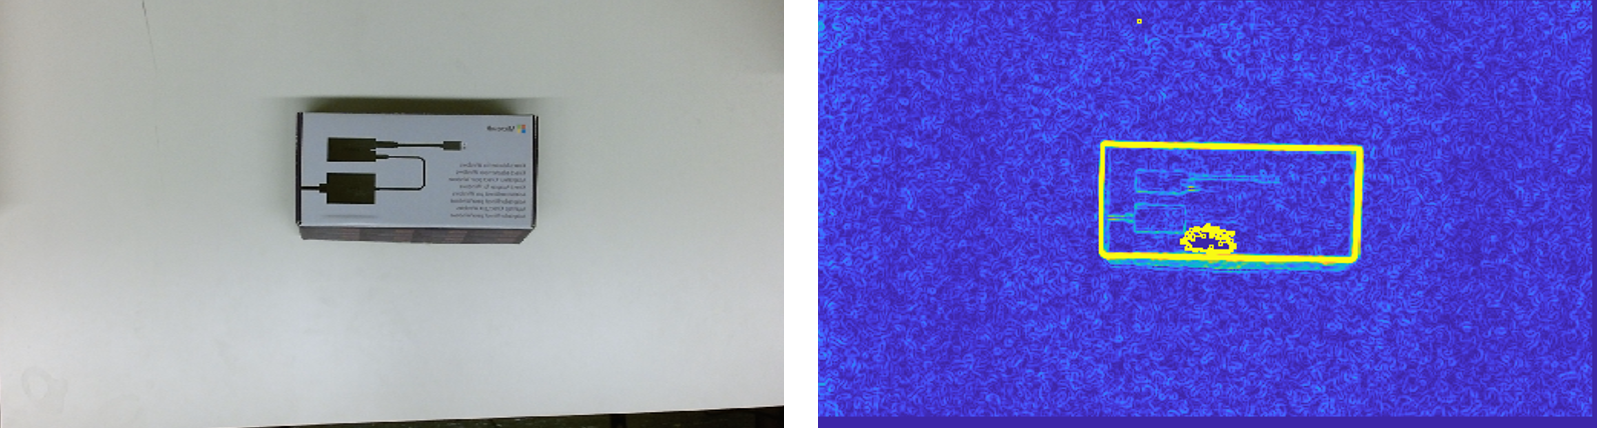
\includegraphics[width=1\linewidth]{original_and_sobel.png}
  \caption{The original RGB image (left) and the image after the Sobel-Feldman operator (right)}
  \label{fig:original_and_sobel}
\end{figure}

\paragraph{Filtering of the noise}\mbox{}\\
After adding al the different magnitudes of the gradients to an array, some anomalies still exist. There can be some impossible elements, like points that seem to be further away than the basket, or fluctuations in areas that are supposed to be flat (noise). The simplest way to solve this problem would be to use a maximum and minimum threshold: The maximum threshold can be a value that is further away than the basket. These values are impossible and the corresponding values in the matrix can be set to zero. The minimum threshold can be decided by empirical research. Values lower than this value can be seen as noise and thus can be set to zero. The final result can be seen in \DIFdelbegin \DIFdel{fig}\DIFdelend \DIFaddbegin \DIFadd{Fig}\DIFaddend . ~\ref{fig:sobel_and_threshold}.

\begin{figure}[h]
	\center
  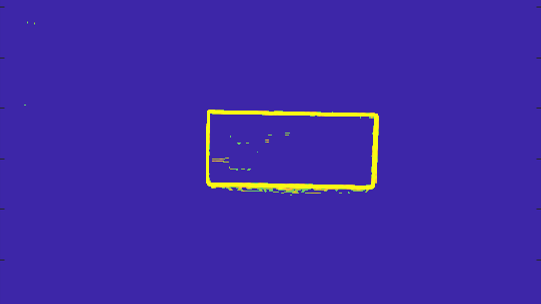
\includegraphics[width=0.6\linewidth]{sobel_and_threshold.png}
  \caption{The original image after using a Sobel-Feldman operator and a threshold filter}
  \label{fig:sobel_and_threshold}
\end{figure}

\section{Research}
An important part of a project is research. Without reading through previous experiences or discoveries within the domain of the project, it will be very hard to figure out a solution. Let alone being comfortable enough in the domain to try something drastically new and (hopefully) develop new ideas in the specific branch of the subject. Although image processing is a recent research domain\DIFdelbegin \DIFdel{. It }\DIFdelend \DIFaddbegin \DIFadd{, it }\DIFaddend is quite popular and already has a lot of foundations to built from. Even Matlab has some predefined functions and libraries to assist the development of image processing software.
However, the goal of this project is to get insight in the programming and working of image processing. To achieve this goal as good as possible, in the end result, there should be \DIFdelbegin \DIFdel{almost no }\DIFdelend \DIFaddbegin \DIFadd{little }\DIFaddend use of predefined functions or libraries. They will only be used if they are completely comprehensible or if they make the code more elegant by doing ordinary operations. 
The next section goes \DIFdelbegin \DIFdel{through the methodology of solving the problem if the use of functions was preferred}\DIFdelend \DIFaddbegin \DIFadd{over a few functions which could be used to build on the already existing program described above. All these functions are explained so they can be implemented manually at a later time}\DIFaddend . It starts by using functions to detect and count the objects, and ends with surrounding the objects with a rectangle, as well as highlighting the edges. \DIFdelbegin %DIFDELCMD < 

%DIFDELCMD < \noindent %%%
\DIFdel{Throughout the project a lot of different approaches were tested and discarded. But in essence, they all do the same thing. En plus, there are functions , delivered in the Image Processing Toolbox which can replace the already finished algorithms. A brief overview of each element is given in the following section}\DIFdelend \DIFaddbegin \DIFadd{An example of these functions can be found in Appendix F}\DIFaddend .

%DIF < They convert the original image to a binary image. Afterwards, this binary array is analysed and a simple algorithm suffices to count the objects. In this %fase of the program the same code is applicable. This code consists of a few important parts: the actual counting and the drawing of the boundary boxes. 
\DIFdelbegin %DIFDELCMD < 

%DIFDELCMD < %%%
\DIFdelend \paragraph{Counting of the objects}\mbox{}\\
The central objective of this paper is counting the amount of objects in a specific rectangular field of view. The general approach to this problem is converting the image to a binary image where black pixels represent the background and white pixels represent the objects. By counting the groups of pixels, it is possible to know how many objects the original image contains. In the image processing toolbox for matlab\cite{Mathworks}, a few functions exist that are very \DIFdelbegin \DIFdel{usefull }\DIFdelend \DIFaddbegin \DIFadd{useful }\DIFaddend for this kind of tasks. One of these functions \DIFaddbegin \DIFadd{called }\DIFaddend bwlabel actually counts group of pixels of at least 8 that are connected. The syntax of this function goes as follows: 
\begin{equation}
[L, num] = bwlabel(BW)
\end{equation}
where BW represents the binary (or black and white) image; num represents the number of objects in the BW image and where L represents a matrix were the first group of pixels are numbered 1, the second group 2 etc. \DIFdelbegin \DIFdel{that way it'}\DIFdelend \DIFaddbegin \DIFadd{That way it’}\DIFaddend s easier to get \DIFdelbegin \DIFdel{a count for }\DIFdelend \DIFaddbegin \DIFadd{an overview of }\DIFaddend how many objects there are.

\paragraph{Boundary boxes}\mbox{}\\
The image processing toolbox really simplifies the drawing of boundary boxes. Once a binary image is obtained\DIFaddbegin \DIFadd{, }\DIFaddend the function regionprops \cite{Mathworks} can extract properties about image regions. Where image regions are defined as 8-connected components in an binary image. This means that each image region contains at least 8 interconnected white pixels, since the black pixels are registered as background. The property that's interesting for this part of the project is called 'boundingbox'. This property returns for every image region the smallest rectangle \DIFdelbegin \DIFdel{containing }\DIFdelend \DIFaddbegin \DIFadd{that contains }\DIFaddend this region. In two dimensions this is a vector with 4 values, the x-coordinate of the upper left corner, the y-coordinate of that corner, the width and the height. The function 
\begin{equation}
rectangle('Position', pos)
\end{equation}
where 'Position' declares the input and where pos is the input obtained from regionprops, can easily display this boundingbox. 

\paragraph{Edge detection}\mbox{}\\
There are a lot of ways to implement edge detection. Edge detection algorithms as described in \DIFdelbegin \DIFdel{PARAGRAPH }\DIFdelend \DIFaddbegin \DIFadd{section 3.2.1 paragraph 4, }\DIFaddend exist for greyscale \DIFdelbegin \DIFdel{image}\DIFdelend \DIFaddbegin \DIFadd{images}\DIFaddend . But if a binary image is available, this becomes much easier. \DIFdelbegin \DIFdel{For starters there exists a function }\DIFdelend \DIFaddbegin \DIFadd{To start, a function called bwboundaries exists }\DIFaddend in the image processing toolbox \DIFdelbegin \DIFdel{called bwboundaries }\DIFdelend \cite{Mathworks}. The syntax of that function goes as follows: 
\begin{equation}
B = bwboundaries (BW)
\end{equation}
where BW represents the input\DIFdelbegin \DIFdel{, this }\DIFdelend \DIFaddbegin \DIFadd{. This }\DIFaddend is a binary image which only consists out of black and white pixels; and B represents the output, which consist out of a cell array with N elements (number of image regions in the binary image), all these elements contain a list of the boundary pixels. Which in turn are fairly easy to draw. They can be inserted in the matrix of the image by replacing values, this is done by looping through the cell arrays. The advantage of this method is that the image can actually be printed. When they are drawn on top of the image with a function like visboundaries\DIFaddbegin \DIFadd{, }\DIFaddend the actual values of the pixels stay unchanged, but it \DIFdelbegin \DIFdel{become different figures }\DIFdelend \DIFaddbegin \DIFadd{different figures arise}\DIFaddend . One with the image and another on top of it with the edges. 
The function bwboundaries implements the Moore-Neighbor tracing algorithm \cite{Moore_Neighborhood}. The algorithm loops through the entire matrix until it finds a white pixel (a pixel that belongs to an image region). This pixel is defined as the start pixel. Once it finds a start pixel it searches for the next connected white pixel. This means another white pixel in one of the eight regions around the start. The algorithm does this by examining the pixels in a clockwise direction. Once it finds a new white pixel, this pixel is added to the sequence B and becomes our new start pixel. This process keeps on running until the algorithm visits the first start pixel for a second time. The only problem with this algorithm is that sometimes the first start pixel is visited for a second time before all of the outline is visited. This is illustrated in Fig.~\ref{fig:Moore_Neighbor}).

\begin{figure}[h]
	\center
  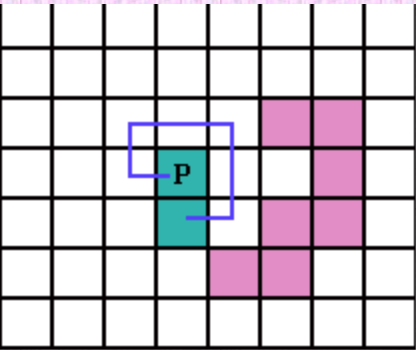
\includegraphics[width=0.3\linewidth]{Moore_Neighbor.png}
  \caption{Problem with stopping criteria Moore-Neighbor tracing algorithm.\DIFaddbeginFL \DIFaddFL{\mbox{%DIFAUXCMD
\cite{Moore_Neighborhood}}\hspace{0pt}%DIFAUXCMD
}\DIFaddendFL }
  \label{fig:Moore_Neighbor}
\end{figure}

\noindent This problem is resolved with the Jacob's stopping criterion. Which states that the algorithm can stop once the first start pixel is visited \DIFdelbegin \DIFdel{out of }\DIFdelend \DIFaddbegin \DIFadd{from }\DIFaddend the same direction as it \DIFdelbegin \DIFdel{was initially }\DIFdelend \DIFaddbegin \DIFadd{initially was }\DIFaddend entered. This leaves four possibilities that need to be checked, from below, from the left, from above or from the right. With this additional criteria, every pixel at the edge of a connected region is visited. 
To find the edges of all the interconnected image regions this process is repeated until every pixel of the image matrix has been checked. 

\section{Further planning}
Being halfway trough the project, a visual timeframe is created. \DIFdelbegin \DIFdel{Appendix D the }\DIFdelend \DIFaddbegin \DIFadd{The }\DIFaddend Gantt chart followed in the project \DIFaddbegin \DIFadd{can be found in Appendix G}\DIFaddend .
This visualizes the current state of the solution for the described problem, as well as the schedule for the next few weeks. 
This project contains five milestones, two of them are already achieved. These have a minor value in prospect to the total paper though. The most important occupancy of the next weeks is implementing key elements of the final algorithm. Key components like filling the edges, creating the boundary boxes and eventually counting the number of objects still need the necessary attention. All of this while the given deadlines need to be respected. As it is possible to view in the chart, the decision to start rather early on the folder is made. A professional representation of the findings takes time. So planning it like this, ensures enough time to perfect the folder. \\
In general, the project is on schedule. From a critical point of view, too much time writing the report during the team sessions was wasted. For the final paper, more individual work is recommended and will happen.

\section{Budget management}
As seen above, the system explained in this paper primarily consists of software which on its own doesn't cost anything. On the contrary, the necessary hardware is rather costly. The current set-up consists of a tripod and the electronics. The tripod is lend for free by the faculty thus the only remaining costs are the Kinect v2 and its adapter to connect with a personal computer.\\
With a budget of \euro 250, this is feasible. Both the Kinect and the adapter have been ordered but as of writing, a fixed price isn't known. At the current market prices, the estimated cost is \euro 200. The remaining \euro 50 are a safe backup for other small costs.

\section{Course Integration}
Solving the problem explained in this report is the main objective of the course P\&O 3 (B-KUL-H01D4B). This course is part of the bachelor in engineering science curriculum of the KU Leuven. It is a course which uses concepts seen in others to solve problems. By now it should be apparent that, indeed, many courses were used to tackle the given problem.\\
Knowledge of linear algebra is applied extensively. Simple concepts like matrix multiplication to more advanced ones like matrix convolution form the core of the \DIFdelbegin \DIFdel{algorithms written }\DIFdelend \DIFaddbegin \DIFadd{written algorithms}\DIFaddend . Numerical Mathematics is useful to get an idea what influence measurement errors have on calculations with large matrices. And this course, together with Applied Informatics, give the tools to investigate the time complexity of the algorithm. The latter course has also helped with grasping the Matlab programming language and environment since general programming concepts are a big part of this project.

\section{Conclusion}
After four weeks of group gatherings, a lot of research has been done and a decent amount of progress was made. The project will be executed by using a Microsoft Kinect version 2. The combination of a depth and RGB sensor at a reasonable cost are some of the decisive arguments over a standard webcam or an industrial camera. \\
When obtaining the image from the RGB sensor, the three dimensional matrix is turned into a one dimensional matrix and thus into a greyscale image. A Gaussian blur and an edge detection algorithm are used to further reduce this matrix to a binary array where only the edges are highlighted. Meanwhile, using a Sobel-Feldman operator and a threshold filter, the image obtained from the depth sensor will become clean with a clearly visible outline around the differences in height. \\
Next, the goal is to, after merging the processed data from the RGB and depth sensor, perfect the positioning of the edges and fill in possible blank spots. Subsequently, a step towards counting the objects will be made. If the amount of progress made per day will stay consistent, all the deadlines should be  accomplished in the given timeframe. But perseverance and a critical point of view are needed to successfully finish this assignment. 

\newpage

\nocite{*}
\bibliographystyle{apacite}
\bibliography{references.bib}
\newpage
\DIFdelbegin \section{\DIFdel{Appendix}}
%DIFAUXCMD
\addtocounter{section}{-1}%DIFAUXCMD
\DIFdelend 

\DIFaddbegin \includepdf[pages=1,scale=.8,pagecommand={\section{Appendices}\subsection*{A: Diagram}\label{pdf:workplan_def}},linktodoc=true]{workplan_def.pdf}

\DIFaddend %%%%% code RGB sensor %%%%%

\lstset{language=Matlab,%
    %basicstyle=\color{red},
    breaklines=true,%
    morekeywords={matlab2tikz},
    keywordstyle=\color{blue},%
    morekeywords=[2]{1}, keywordstyle=[2]{\color{black}},
    identifierstyle=\color{black},%
    stringstyle=\color{mylilas},
    commentstyle=\color{mygreen},%
    showstringspaces=false,%without this there will be a symbol in the places where there is a space
    numbers=left,%
    numberstyle={\tiny \color{black}},% size of the numbers
    numbersep=9pt, % this defines how far the numbers are from the text
    emph=[1]{for,end,break},emphstyle=[1]\color{blue}, %some words to emphasise
    %emph=[2]{word1,word2}, emphstyle=[2]{style},    
}

\DIFaddbegin \newpage
\DIFaddend \subsection*{\DIFdelbegin \DIFdel{A}\DIFdelend \DIFaddbegin \DIFadd{B}\DIFaddend : Matlab Threshold Functions }
\lstinputlisting{threshold.m}

\newpage

\subsection*{\DIFdelbegin \DIFdel{B}\DIFdelend \DIFaddbegin \DIFadd{C}\DIFaddend : Matlab Erasing Background}
\lstinputlisting{histogram.m}

\newpage
\DIFdelbegin %DIFDELCMD < 

%DIFDELCMD < %%%
\DIFdelend \subsection*{\DIFdelbegin \DIFdel{C}\DIFdelend \DIFaddbegin \DIFadd{D}\DIFaddend : Matlab Code RGB Sensor}
\lstinputlisting{image_processing_week4.m}

\newpage
\subsection*{\DIFdelbegin \DIFdel{D}\DIFdelend \DIFaddbegin \DIFadd{E}\DIFaddend : Matlab Code Septh Sensor}
\lstinputlisting{testDepth.m}

\newpage
\subsection*{\DIFdelbegin \DIFdel{E}\DIFdelend \DIFaddbegin \DIFadd{F}\DIFaddend : Matlab Library Functions}
\lstinputlisting{extra_functionalities.m}

\newpage
\DIFdelbegin %DIFDELCMD < \includepdf[pages=1,scale=.8,pagecommand={\subsection*{F: Diagram}\label{pdf:workplan_def}},linktodoc=true]{workplan_def.pdf}
%DIFDELCMD < 

%DIFDELCMD < \newpage
%DIFDELCMD < 

%DIFDELCMD < %%%
\DIFdelend 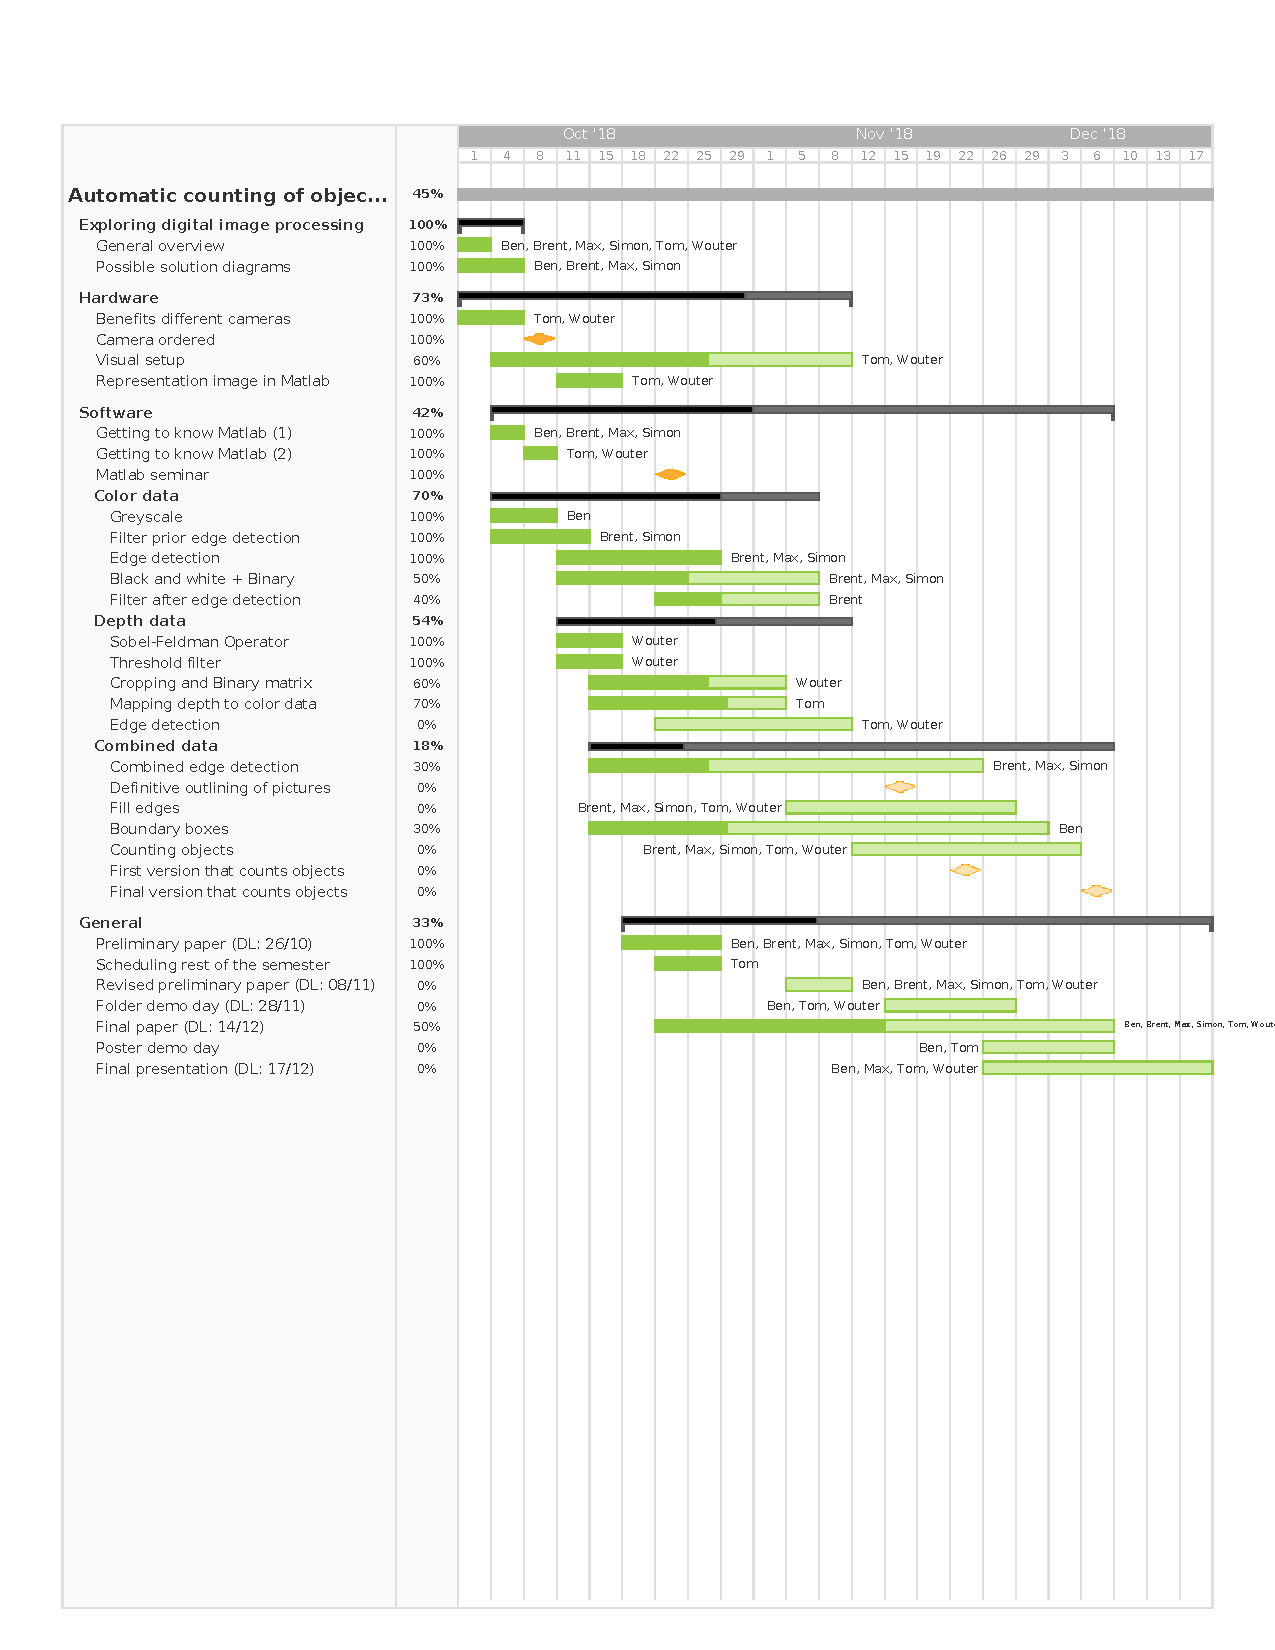
\includepdf[scale=.8,pagecommand={\subsection*{G: Gantt chart}\label{pdf:Auto}},linktodoc=true]{Auto.pdf}

\end{document}
